% Exam Template for UMTYMP and Math Department courses
%
% Using Philip Hirschhorn's exam.cls: http://www-math.mit.edu/~psh/#ExamCls
%
% run pdflatex on a finished exam at least three times to do the grading table on front page.
%
%%%%%%%%%%%%%%%%%%%%%%%%%%%%%%%%%%%%%%%%%%%%%%%%%%%%%%%%%%%%%%%%%%%%%%%%%%%%%%%%%%%%%%%%%%%%%%

% These lines can probably stay unchanged, although you can remove the last
% two packages if you're not making pictures with tikz.
\documentclass[11pt]{exam}
\RequirePackage{amssymb, amsfonts, amsmath, latexsym, verbatim, xspace, setspace}
\RequirePackage{tikz, pgflibraryplotmarks}

% By default LaTeX uses large margins.  This doesn't work well on exams; problems
% end up in the "middle" of the page, reducing the amount of space for students
% to work on them.
\usepackage[margin=1in]{geometry}
\usepackage{afterpage}
\usepackage{changepage}
\usepackage{hyperref}

% Here's where you edit the Class, Exam, Date, etc.
\newcommand{\class}{CS 143A}
\newcommand{\term}{Fall 2018}
\newcommand{\examnum}{Midterm}
\newcommand{\examdate}{11/15/2018}
\newcommand{\timelimit}{2:00pm - 3:20pm}

% For an exam, single spacing is most appropriate
\singlespacing
% \onehalfspacing
% \doublespacing

% For an exam, we generally want to turn off paragraph indentation
\parindent 0ex

\begin{document} 

% These commands set up the running header on the top of the exam pages
\pagestyle{head}
\firstpageheader{}{}{}
\runningheader{\class}{\examnum\ - Page \thepage\ of
\numpages}{\fbox{\rule{2in}{0pt}\rule[-0.5ex]{0pt}{5ex}}}
\runningheadrule

\begin{flushright}
\begin{tabular}{p{2.8in} r l}
%\textbf{\class} & \textbf{Name (Print):} & \makebox[2in]{\hrulefill}\\
  \textbf{\class} & \textbf{Name (Print):} &
  \fbox{\rule{2in}{0pt}\rule[-0.5ex]{0pt}{5ex}}\\
\textbf{\term} &&\\
\textbf{\examnum} &&\\
\textbf{\examdate} &&\\
\textbf{Time Limit: \timelimit} & & \\
\end{tabular}\\
\end{flushright}
\rule[1ex]{\textwidth}{.1pt}




%\begin{minipage}[t]{3.7in}
%\vspace{0pt}
\begin{itemize}

\item \textbf{Don't forget to write your name on this exam.} 

\item \textbf{This is an open book, open notes exam. But no online or 
    in-class chatting.  } 

    
\item \textbf{Ask us if something is confusing in the questions.}

\item \textbf{Organize your work}, in a reasonably neat and coherent way, in
the space provided. Work scattered all over the page without a clear ordering will 
receive very little credit.  

\item \textbf{Mysterious or unsupported answers will not receive full
credit}.  A correct answer, unsupported by explanation will receive no credit; 
an incorrect answer supported by substantially correct explanations might still 
receive partial credit.

\item If you need more space, use the back of the pages; clearly indicate when you have done this.
\end{itemize}

%Do not write in the table to the right.
%\end{minipage}
%\hfill

%\begin{minipage}[t]{2.3in}
%\vspace{0pt}
%\cellwidth{3em}
%\gradetablestretch{2}
\vqword{Problem}
\addpoints % required here by exam.cls, even though questions haven't started yet.	
\gradetable[v]%[pages]  % Use [pages] to have grading table by page instead of question

%\end{minipage}
\newpage % End of cover page

%%%%%%%%%%%%%%%%%%%%%%%%%%%%%%%%%%%%%%%%%%%%%%%%%%%%%%%%%%%%%%%%%%%%%%%%%%%%%%%%%%%%%
%
% See http://www-math.mit.edu/~psh/#ExamCls for full documentation, but the questions
% below give an idea of how to write questions [with parts] and have the points
% tracked automatically on the cover page.
%
%
%%%%%%%%%%%%%%%%%%%%%%%%%%%%%%%%%%%%%%%%%%%%%%%%%%%%%%%%%%%%%%%%%%%%%%%%%%%%%%%%%%%%%

\begin{questions}

% Basic question
\addpoints
\question OS Interfaces 

\begin{parts}
 
\part[5] Here’s a program that uses the UNIX system call API, as described in Chapter 0 of the xv6 book:
\begin{verbatim}
#include "param.h"
#include "types.h"
#include "user.h"
#include "syscall.h"

int main() {
  char * message = "aaa\n";
  int pid = fork();
  
  if(pid != 0){

    char *echoargv[] = { "echo", "Hello\n", 0 };
    
    message = "bbb\n";
    exec("echo", echoargv);
    write(1, message, 4); 

  }

  write(1, message, 4);
  exit();
}
\end{verbatim}

Assume that fork() succeeds, that file descriptor 1 is connected to the
terminal when the program starts, and \texttt{echo} program exists. What
possible outputs this program can produce (explain your answer)?  

Answer: The proccess forks() and execs() the ``echo'' program that prints ``Hello''
inside the parent. Since exec() overloads the address space of the parent the write(1, message, 4)line never gets executed (we assume that ``echo'' exists and exec() succeeds). The child 
prints ``aaa''. Two possible outputs depending on the order in which parent and child execute 
are 

\begin{verbatim}
aaa
Hello
\end{verbatim}

or

\begin{verbatim}
Hello
aaa
\end{verbatim}


\vfill

\newpage

\part[10] 

Write a program that uses the UNIX system call API, as described in Chapter 0
of the xv6 book. The program forks and creates a pipeline of 10 stages.
I.e., each stage is a separate process. Each two consequtive stages are
connected with a pipe, i.e., the standard output of each stage is connected to the 
standard input of the next stage. Each stage reads a character from its standard
input and sends it to the standard output. The last stage outputs the
character it reads from the pipe to the standard output. 

\textbf{STUDENT SOLUTION } 
\begin{adjustwidth}{1.5em}{1em}
Please see the C file at \href{https://github.com/StrayBird-ATSH/OperatingSystemCourseMidTermExams/blob/master/Fall\%202018/Fall2018Mid-TenLevelPipe.c}{this file}
\end{adjustwidth}
\vfill

\vfill 


\end{parts} 

% Basic question
\addpoints

\newpage
\question Basic page tables.

\begin{parts}
\part[5] 

Alice wants to construct a page table that maps virtual addresses 0x0, 0x1000
and 0x2000 into physical addresses 0x1000, 0x2000, and 0x3000. Assume that the
Page Directory Page is at physical address 0x0, and the Page Table Page is at
physical address 0x00001000 (which is PPN 0x00001). 

Draw a picture of the page table Alice will construct (or alternatively simply
write it down in the format similar to the one below): : 

Page Directory Page:

\begin{verbatim}
PDE 0: PPN=0x1, PTE_P, PTE_U, PTE_W
\end{verbatim}

... all other PDEs are zero

The Page Table Page:

\begin{verbatim}
PTE 0: PPN=0x1, PTE_P, PTE_U, PTE_W
PTE 1: PPN=0x2, PTE_P, PTE_U, PTE_W
PTE 2: PPN=0x3, PTE_P, PTE_U, PTE_W
\end{verbatim}

... all other PTEs are zero

\end{parts} 

\textbf{STUDENT SOLUTION } 
\begin{adjustwidth}{1.5em}{1em}
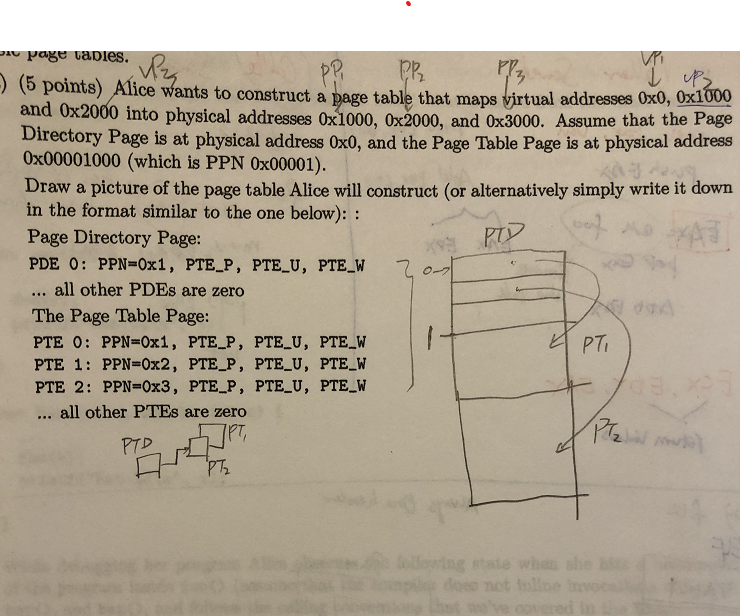
\includegraphics[width=0.5\columnwidth]{figs/point-2a-ans}
\end{adjustwidth}
\vfill

\newpage \addpoints

\question Stack and calling conventions. 

Alice developed a program that has a function \texttt{foo()} that is called
from two other functions \texttt{bar()} and \texttt{baz()}:

\begin{verbatim}
int foo(int a) {
  ...
}

int bar(int a, int b) {
  ...
  foo(x);
  printf("bar:\%d\n", x); 
  ...
}

int baz(int a, int b, int c) {
  ...
  foo(x);
  printf("baz:\%d\n", x);
  ...
}
\end{verbatim}

While debugging her program Alice observes the following state when she hits a breakpoint of the 
program inside \texttt{foo()} (assume that the compiler does not inline invocations of \texttt{foo()}, 
\texttt{bar()}, and \texttt{baz()}, and follows the calling conventions that we've covered in the class):

\begin{verbatim}
The bottom of the stack:

0x8010b5b4: ... 
0x8010b5b0: 0x00000003
0x8010b5ac: 0x00000002 
0x8010b5a8  0x80102e80 
0x8010b5a4: 0x8010b5b4 
0x8010b5a0: 0x80112780 
0x8010b59c: 0x00000001 
0x8010b598: 0x80102e32 
0x8010b594: 0x8010b5a4    <-- ebp
0x8010b590: 0x00000000    <-- esp
\end{verbatim}

\begin{parts} 

\part[5] Provide a short explanation for each line of the stack dump above (you can annotate the printout above). 

\begin{verbatim}
The bottom of the stack:

0x8010b5b4: ...        // ebp
0x8010b5b0: 0x00000003 // argument #2 to the function that called foo()'s caller
0x8010b5ac: 0x00000002 // argument #1 to the function that called foo()'s caller
0x8010b5a8  0x80102e80 // return address
0x8010b5a4: 0x8010b5b4 // ebp
0x8010b5a0: 0x80112780 // (local variable, argument to a funciton, or register spill inside function that called foo) 
0x8010b59c: 0x00000001 // arg to foo	
0x8010b598: 0x80102e32 // return address for foo()
0x8010b594: 0x8010b5a4    <-- ebp
0x8010b590: 0x00000000    <-- esp (local variable, argument to a funciton, or register spill inside foo)
\end{verbatim}

\newpage
\part[5] If Alice continues execution of her program what output will she see on the screen (justify your answer).  

We know that foo() can be called from bar() or baz(), but we also know that the caller of foo()'s caller i.e., either bar() or baz(), got two arguments. Hence, it's bar(). And since we know that 
foo() got 0x1 as argument the string Alice will see on the screen should be

\begin{verbatim}
bar:1
\end{verbatim}

\vfill



\end{parts}


\addpoints

\question Xv6 process organization. 

In xv6, in the address space of the process, what does the following virtual addresses contain? 

\begin{parts} 

\part[3] Virtual address 0x0

The memory at virtual address 0x0 contains the text section (code) of the user process.  
\vfill

\part[3] Virtual address 0x80100000

The memory at virtual address 0x80100000 contains the text section (code) of the kernel. During 
the boot the kernel was loaded at physical address 0x100000 (1MB) and then later this address was mapped at 2GBs + 1MB or (0x80000000 + 0x100000).   

\vfill

\part[3] What physical address is mapped at virtual address 0x80000000

Physical address 0x0. 

\vfill


\newpage

\part[7] Is there a way for the kernel to find out what physical address is
mapped at a specific virtual address? Provide an explanation and a code sketch
(pseudocode is ok, no need to worry about correct C syntax). Your code should
take a virtual address as an input and resolve it into the physical address
that is mapped into that virtual address by the process page table (in your
code feel free to re-use functions that are already implemented in the xv6
kernel).  

\textbf{STUDENT SOLUTION } 
\begin{adjustwidth}{1.5em}{1em}

In xv6 we can access the entire page table and the page tables contain information about how a virtual address maps to the physical address. Therefore, we only need to go though the table to find out where the physical page lie in the page table and then we will be able to find out the virtual addresses that are directing to this physical address.

Please see the C file at 
\href{https://github.com/StrayBird-ATSH/OperatingSystemCourseMidTermExams/blob/master/Fall\%202018/Fall2018Mid-Virtual2Physical.c}{this file}

\end{adjustwidth}
\vfill


\end{parts}


\newpage

\addpoints 

\question Protection and isolation

\begin{parts}

\part[5] In xv6 all segments are configured to have the base of 0 and limit of
4GBs, which means that segmentation does not prevent user programs from
accessing kernel memory.  Nevertheless, user programs can't read and write
kernel memory. How (through what mechanisms) such isolation is achieved?

\textbf{STUDENT SOLUTION } 
\begin{adjustwidth}{1.5em}{1em}
Above all, xv6 adopts page tables. That is, the kernel memory and user memory will reside in different pages. Also, each page has a flag indicating whether this page is for kernel or for user. Therefore, when a user program wants to access kernel program, it will access the kernel pages, and visiting a page with a kernel flag will trigger a fault. So achieved.
  
\end{adjustwidth}
\vfill

\end{parts}

\addpoints

\question System calls

\begin{parts}

\part[5] How do system calls access their arguments that are passed from the
user level? After all, all system calls are declared as void functions that
return an integer, i.e., visibly they don't take any arguments. For example,
the \texttt{read()} system call is declared as:

\begin{verbatim} 
6131 int 
6132 sys_read(void) 
\end{verbatim}

But user code can invoke it as 

\begin{verbatim}
int read(int, void*, int);
\end{verbatim}

\vfill


\part[5] Rudi What is the significance of the line 6138 in the listing below (\texttt{sys\_read()} is the xv6 system 
call that reads data from the file pointed by the file descriptor passed as the first argument,  

\begin{verbatim}
6131 int
6132 sys_read(void)
6133 {
6134   struct file *f;
6135   int n;
6136   char *p;
6137 
6138   if(argfd(0, 0, &f) < 0 || argint(2, &n) < 0 || argptr(1, &p, n) < 0)
6139     return -1;
6140   return fileread(f, p, n);
6141 }
\end{verbatim} 

\textbf{STUDENT SOLUTION } 
\begin{adjustwidth}{1.5em}{1em}
source code is syscall.c , below is the explaination from syscall.c comments about how system calls get arguments.
\begin{verbatim}
// User code makes a system call with INT T\_SYSCALL.
// System call number in \%eax.
// Arguments on the stack, from the user call to the C
// library system call function. The saved user \%esp points
// to a saved program counter, and then the first argument.
// Fetch the int at addr from the current process.
  \end{verbatim} 
\end{adjustwidth}

\end{parts}


% Question with parts
\newpage
\addpoints 

\question Physical and virtual memory allocation

\begin{parts} 

\part[5] What is the purpose of the V2P macro? Specifically, the \texttt{allocuvm()} function (see the listing below) 
uses \texttt{kalloc()} to allocate and map a region of memory into the address space 
of a process. Explain, why the \texttt{V2P} macro is used in line 1946 below? 

\begin{verbatim}

1926 int
1927 allocuvm(pde_t *pgdir, uint oldsz, uint newsz)
1928 {
1929   char *mem;
1930   uint a;
1931 
1932   if(newsz >= KERNBASE)
1933     return 0;
1934   if(newsz < oldsz)
1935     return oldsz;
1936 
1937   a = PGROUNDUP(oldsz);
1938   for(; a < newsz; a += PGSIZE){
1939     mem = kalloc();
1940     if(mem == 0){
1941       cprintf("allocuvm out of memory\n");
1942       deallocuvm(pgdir, newsz, oldsz);
1943       return 0;
1944     }
1945     memset(mem, 0, PGSIZE);
1946     if(mappages(pgdir, (char*)a, PGSIZE, V2P(mem), PTE_W|PTE_U) < 0){
1947       cprintf("allocuvm out of memory (2)\n");
1948       deallocuvm(pgdir, newsz, oldsz);
1949       kfree(mem)
1950       return 0;
1951     }
1952   }
1953   return newsz; 
1954 }

\end{verbatim}

\textbf{STUDENT SOLUTION } 
\begin{adjustwidth}{1.5em}{1em}
It translates a virtual address into physical address.  
  
Because the mappages needs to check whether a physical page is mapped or not, or whether it is available. This translations gives the mappages function the location of the physical page needed and this function will do the mapping work.
  
\end{adjustwidth}
\vfill

\newpage

\begin{verbatim}

\end{verbatim}

\vfill


Bob looks at the \texttt{clearpteu()} function in the xv6 kernel (see below) and decides that invocation of the \texttt{walkpgdir()} function is not necessary. He knows that xv6 defines the V2P macro, and hence he believes that it's ok to use it instead oto implement 


Bob decides to enable xv6 with the ability to share their memory with each other. I.e., a process can register a region of its memory with the kernel, and later any other process can map that region into its own address space. Bob develops a new system call that registers a region of process' memory with the kernel (here. Later, any other process can 

\begin{verbatim}
void
sys_share(char name[32], char *uva, int size)
{
  
  
  
  pa = V2P(uva);
  
}
\end{verbatim}

\textbf{STUDENT SOLUTION } 
\begin{adjustwidth}{1.5em}{1em}
Because when the system initially boots, there was no kernel section in the upper 2GB and the codes are in the first 4MB space. Therefore, before the new page table is successfully mapped, we still need the mapping of the first 4MB to keep the code running smoothly.
  
  
\end{adjustwidth}
\vfill

\end{parts} 

%\newpage 

\addpoints

\question Initial page tables

Bob looks at the piece of code in entry.S where the initial page tables are
set and thinks he doesn't need the entry that maps the 0-4MB of virtual
page to 0-4MB of physical page. Accordingly he modifies the entrypgdir as
below.

\begin{verbatim}
__attribute__((__aligned__(PGSIZE)))
pde_t entrypgdir[NPDENTRIES] = {
  // Map VA's [KERNBASE, KERNBASE+4MB) to PA's [0, 4MB)
  [KERNBASE>>PDXSHIFT] = (0) | PTE_P | PTE_W | PTE_PS,
};
\end{verbatim}


\begin{parts} 

\part[5] Explain what will go wrong with Bob's change?

\textbf{STUDENT SOLUTION } 
\begin{adjustwidth}{1.5em}{1em}
Because when the system initially boots, there was no kernel section in the upper 2GB and the codes are in the first 4MB space. Therefore, before the new page table is successfully mapped, we still need the mapping of the first 4MB to keep the code running smoothly.
   
\end{adjustwidth}
\vfill

\end{parts}

\newpage

\addpoints
\question 143A organization and teaching

\begin{parts} 

\part[3] If there is one single most important thing you would like to improve in 
the CS143A class, what would it be? 


\vfill

\end{parts}


\end{questions}
%\afterpage{\null\newpage}
\afterpage{\null\newpage}
\end{document}
